\section{Problemas a abordar}

El principal objetivo de este trabajo fin de grado es dar soporte dentro de la plataforma software
JdeRobot a drones que utilicen el protocolo MAVLink para comunicarse con la controladora a bordo. Este problema lo hemos dividido varios subobjetivos:

\begin{enumerate}
\item Desarrollar un driver para pilotar drones usando una interfaz de comandos de velocidad. Se comunicará con el dron usando el protocolo MavLink y ofrecerá el interfaz de nivel medio que ya existe en JdeRobot para manejar drones llamada CMDVel.
\item Desarrollar una herramienta que permita pilotar los drones usando interfaz de comandos de velocidad en Python de manera intuitiva. Permitira visualizar los datos de los sensores a bordo y la teleoperación del drone de modo similar a los mandos físicos actuales. Esta herramienta será una evolución mejorada de la ya existente que facilita JdeRobot. Será compatible con el driver del primer subobjetivo.
\item Experimentos en dron real. Validaremos experimentalmente ambos desarrollos con un drone 3DR Solo, tanto el driver, como la herramienta renovada de teleoperación que nos permitirá pilotarlo.
\end{enumerate}


\section{Requisitos}

Adicionalmente, como requisitos no funcionales del software a desarrollar tenemos:

\begin{enumerate}
\item Serán programados en lenguaje Python, tanto el driver como la herramienta de teleoperación.
\item Serán multiplataforma que valgan para muchos modelos de drones.
\item Se utilizarán únicamente librerías de software libre y serán software libre.
\item Serán 100 \% compatibles con los actuales interfaces existentes JdeRobot y con la versión 5.6.3 de esa plataforma.
\item Se intregrarán en el repositorio oficial de JdeRobot en GitHub para su uso por terceros.

\end{enumerate}

\section{Metodología}

Durante el ciclo de vida del proyecto se han llevado a cabo reuniones semanales de seguimiento con el tutor. En ellas se evaluaban las tareas realizadas y se marcaba qué dirección tomar para la siguiente iteración o incremento. Si los puntos marcados en la anterior reunión no se habían alcanzado se ampliaba el plazo o se discutían otras vías para avanzar. En caso contrario se proponían nuevos subobjetivos.

Para apoyarnos en nuestro desarrollo hemos utilizado principalmente 3 herramientas metodológicas:
\begin{itemize}
\item GitHub como forja y control de versiones. En el repositorio \footnote{\url{https://github.com/RoboticsURJC-students/2016-tfg-Diego-Jimenez}}
se almacenan todos los desarrollos que son objetivo de este TFG así como esta memoria. También se encuentran subproductos de desarrollo que han ido surgiendo como apoyo o pruebas a los desarrollos principales.
\item Contamos también con un mediawiki en la web de JdeRobot dónde hemos actualizado periódicamente nuestros avances acompañados con explicaciones, vídeos e imágenes. \footnote{\url{http://jderobot.org/Jimenez-tfg}}
\item Todos los vídeos del mediawiki han sido compartidos en Youtube.
\end{itemize}

Se propuso un desarrollo en espiral. Para ello se proponían semanalmente reuniones con el tutor, en las cuales se presentaban unos objetivos a seguir en función de lo que se había conseguido hasta el momento. Una vez propuestas estas tareas se evaluaban los distintos riesgos que se podían tomar en función de trabajar de una forma u otra, y los avances a los que se podía llegar por cada camino. Una vez hecho esto, se comenzaban a desarrollar los algoritmos para conseguir estos objetivos en función de la forma elegida. Después se probaban en el robot real. Por último se proponía otra reunión para determinar si los avances eran los deseados o no, y en función de esto proponer los nuevos objetivos.


\begin{figure}[H]
	\centering
		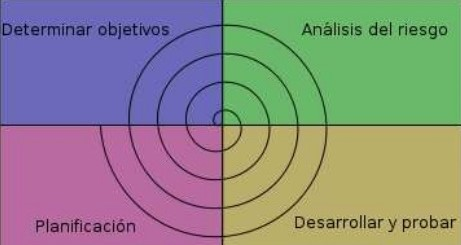
\includegraphics{imagenes/metodologia-espiral.jpg}
        \caption{Método de desarrollo en espiral}
	\label{fig:Desarrollo en espiral}
\end{figure}


\section{Plan de trabajo}
La planificación seguida en el desarrollo ha incluido las siguientes fases:

\begin{itemize}
\item{Formación:} Comprender las distintas herramientas de JdeRobot y trabajar con ellas, creando programas simples y viendo que funcionaban, así como trabajar con distintos robots reales para tener una toma de contacto con ellos. 

\item{EStudio del protocolo MavLink:} Familiarizarse con sus librerías, interfaces y código que se encuentra en el repositorio oficial de ArduPilot \footnote{\url{https://github.com/ArduPilot/MAVProxy}}.

\item{Desarrollo del driver e integración con JdeRobot:} Aprovechar al máximo las funciones que puede desempeñar un dron a través del protocolo MavLink y construir un interfaz ICE en JdeRobot que sea capaz de manejarlo.

\item{Desarrollo de una aplicación de control en tierra:} Para visualizar los datos sensoriales a bordo y para enviar al drone en tiempo real órdenes directas de movimiento a través de un interfaz visual que sea lo más intuitiva posible.

\item{Validación experimental:} Tras marcar un objetivo, se procede al desarrollo y su posterior prueba y ajuste experimental. Una vez concluido y validado, se comienza un nuevo subobjetivo.

\end{itemize}
